We used signal file {\tt Q1\_K2013\_44814P.wav} and chose to do
assignment B, i.e., uncovering the embedded signal and performing the
tasks as instructed in the signal. 

The spectrogram of the original signal, as depicted in
figure \ref{fig:q1_spectrogram}, shows three distinct bands of signals:
0-5kHz, 5kHz-12.5kHz and 12.5kHz-22kHz.

\begin{figure}
  \begin{center}
    \hspace*{-1in}
    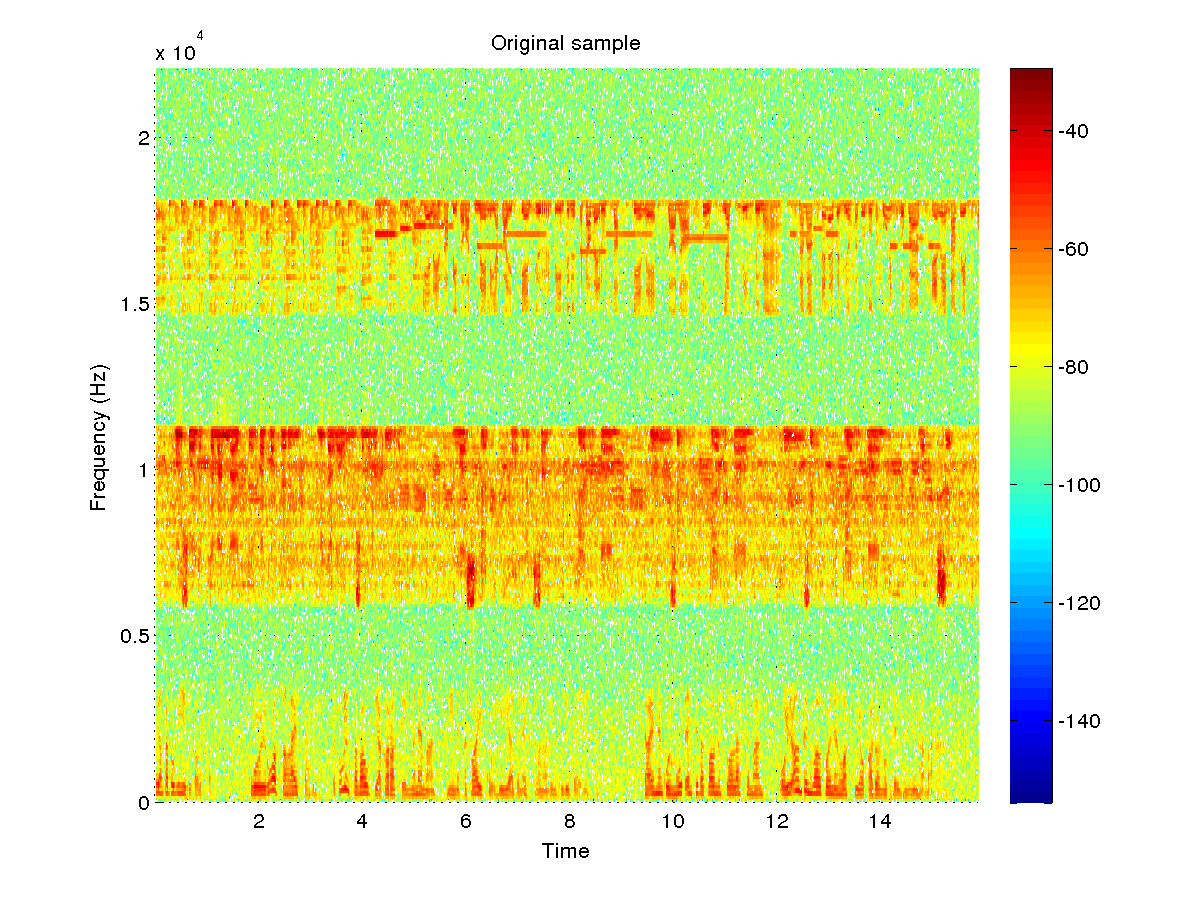
\includegraphics[width=180mm]{q1_spectrogram}
    \caption{Spectrogram of the signal. \label{fig:q1_spectrogram}}
  \end{center}  
\end{figure}

Assignment instructed the use of an IIR-filter with 500Hz transition
bands and maximum of 2 dB passband ripple.  The filter specification was
drawn with {\tt speksitIIR}, obtained from the course page.  The filter
specification is depicted in figure \ref{fig:q1_filter_specification}.

As the IIR filter, we chose Chebyshev type II, because of its good
features for the task at hand, i.e., non-existent ripple in the
passband.

The filtered signal's spectrogram is shown in figure
\ref{fig:q1_filtered_spectrogram}.

\begin{figure}
  \begin{center}
    \hspace*{-1in}
    \includegraphics[width=180mm]{q1_filter_specification}
    \caption{IIR filter specification for the
      passband. \label{fig:q1_filter_specification}}
  \end{center}  
\end{figure}

\begin{figure}
  \begin{center}
    \hspace*{-1in}
    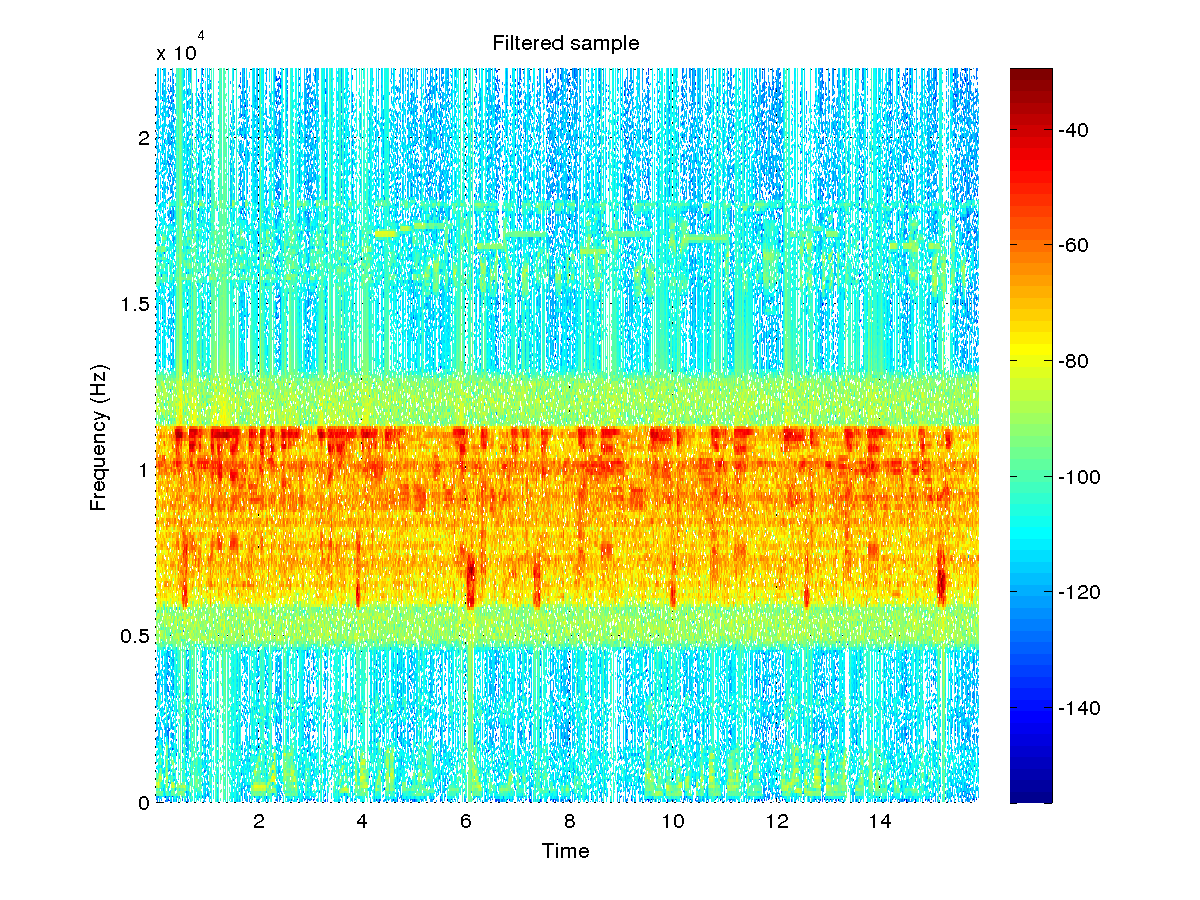
\includegraphics[width=180mm]{q1_filtered_spectrogram}
    \caption{Spectrogram of the filtered signal. 
      \label{fig:q1_filtered_spectrogram}}
  \end{center}  
\end{figure}

Demodulation was done as shown in Matlab round 5, with the following code
\begin{verbatim}
  x_demod = filtered .* cos(2*pi*fc/fT*[1:length(filtered)]');
\end{verbatim}

A nice frequency to perform the demodulation around, 11195 Hz, was found
after a few tries.  This gave a clear signal to listen to.

The sample contains two assignments: writing the song lyrics of the song
that can be heard when the sample is played backwards and the
calculation of ``8 * 6 * 6 * 2''.

The calculation produces the result 576.  The song lyrics can be heard
by using {\tt flipud}, and they are part of a song ``Tuntematon
potilas'' by Arttu Wiskari\cite{wiskari2010}.

\begin{quotation}
eikö aikani täynnä jo ois

olen jo nähnyt tämän elämän

kaiken sain ja vielä enemmän

kuule mun toive

mä haluan pois
\end{quotation}

Matlab code for the assignment is included in appendix \ref{sect:q1m}.
